
\section*{Experience}
%%%%%%%%%%%%%%%%%%%%%%%%%%%%%%

\begin{center}
    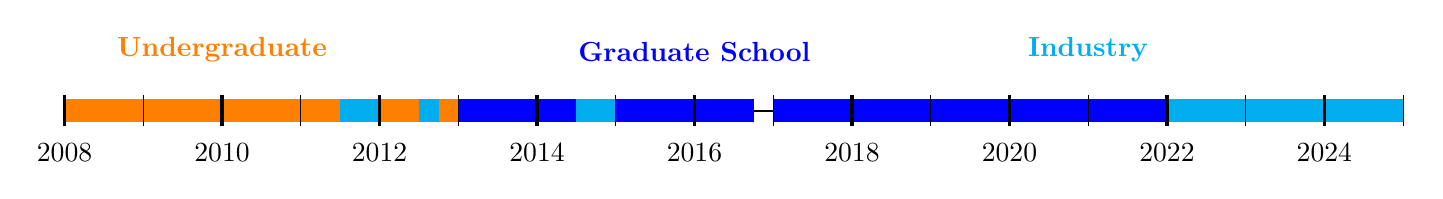
\begin{tikzpicture}
        % Labels above timeline
        \node[above, orange] at (2,0.5) {\textbf{Undergraduate}};
        \node[above, blue] at (8,0.5) {\textbf{Graduate School}};
        \node[above, cyan] at (13,0.5) {\textbf{Industry}};
        
        % Full timeline base (thin gray for reference)
        \draw[thick, black] (0,0) -- (17,0); 
        % Graduate School section (Blue, thicker)
        \draw[line width=3mm, orange] (0,0) -- (5,0);
        \draw[line width=3mm, blue] (5,0) -- (8.75,0);
        \draw[line width=3mm, blue] (9,0) -- (14,0);
        % Industry section (Green, thicker)
        \draw[line width=3mm, cyan] (3.5,0) -- (4,0);
        \draw[line width=3mm, cyan] (4.5,0) -- (4.75,0);
        \draw[line width=3mm, cyan] (6.5,0) -- (7,0);
        \draw[line width=3mm, cyan] (14,0) -- (17,0);
        % Add year markers
        \foreach \x/\year in {0/2008, 2/2010, 4/2012, 6/2014, 8/2016, 10/2018, 12/2020, 14/2022, 16/2024} {
            \draw[very thick] (\x,0.2) -- (\x,-0.2);
            \node[below] at (\x,-0.3) {\year};
        }
        \foreach \x/\year in {1/2009, 3/2011, 5/2013, 7/2015, 9/2017, 11/2019, 13/2021, 15/2023, 17/2025} {
            \draw[line width=0.1mm] (\x,0.2) -- (\x,-0.2);
            {\year};
        }
    \end{tikzpicture}
\end{center}


% \begin{center}
%     \begin{tikzpicture}
%         % Full timeline base (thin gray for reference)
%         \draw[thick, black] (-1,0) -- (12,0); 
%         % Graduate School section (Blue, thicker)
%         \draw[line width=3mm, blue] (0,0) -- (9,0);
%         % Industry section (Green, thicker)
%         \draw[line width=3mm, cyan] (9,0) -- (12,0);
%         % Add year markers
%         \foreach \x/\year in {0/2013, 2/2015, 4/2017, 6/2019, 8/2021, 10/2023, 12/2025} {
%             \draw[very thick] (\x,0.2) -- (\x,-0.2);
%             \node[below] at (\x,-0.3) {\year};
%         }
%         \foreach \x/\year in {-1/2012, 1/2014, 3/2016, 5/2018, 7/2020, 9/2022, 11/2024} {
%             \draw[line width=0.1mm] (\x,0.2) -- (\x,-0.2);
%             {\year};
%         }
%         % Labels above timeline
%         \node[above, blue] at (4,0.6) {\textbf{Graduate School}};
%         \node[above, cyan] at (10,0.6) {\textbf{Industry}};

%     \end{tikzpicture}
% \end{center}


% Job title / role
\newcommand{\JobTitle}[1]{\textbf{#1}}
% Company / organization
\newcommand{\Company}[1]{\textit{#1}}
% Location and dates (aligned right)
\newcommand{\JobDates}[1]{\hfill\textit{#1}}
% Optional: small separator
\newcommand{\JobEntry}[3]{%
  \JobTitle{#1} \JobDates{#3}\\
  \Company{#2}\\
}

\newcommand{\Job}[5]{%
  \noindent\textbf{#1} \hfill \textit{#4}\\
  \textbf{\href{#2}{#3}}\\
  \begin{addmargin}[1cm]{2cm}
    #5
  \end{addmargin}
  \sectionvspace
}
\newcommand{\JobItem}[1]{\item #1}

% -------------------------------
% EXPERIENCE
% -------------------------------

\Job
  {Bioinformatics Senior Computational Scientist}
  {https://nutrienagsolutions.com/}
  {Nutrien Ag Solutions (Waypoint Analytical) | Soil Biome | Champaign, Illinois}
  {Jan 2022 – Present}
  {
    \begin{itemize}[left=-0.2cm, itemsep=-0.15cm]
      \JobItem{Designed and implemented end-to-end NGS pipelines, processing metagenomic datasets at scale.}
      \JobItem{Developed and deployed NextFlow workflows on AWS and GCP to enable reproducible cloud-based analyses.}
      \JobItem{Engineered custom \CC\ software for high-throughput lab data processing and quality control.}
      \JobItem{Authored R and Python packages for advanced microbiome analytics, improving analysis efficiency by 30\%.}
      \JobItem{Managed and curated databases for laboratory and computational teams, ensuring data integrity and accessibility.}
      \JobItem{Built automated soil-biome report generation platform, streamlining client reporting.}
      \JobItem{Implemented predictive models for product-placement using microbiome metrics and machine learning.}
      \JobItem{Developed RAG and GenAI chatbot applications to support internal data queries.}
      \JobItem{Designed and maintained gRPC server architecture for robust API-based data access.}
      \JobItem{Led metagenomic results discovery database project, coordinating a team of 3 developers.}
      \JobItem{Produced stakeholder-ready analyses, visualizations, and presentations for strategic decision-making.}
      \JobItem{Mentored 5+ junior colleagues and summer interns, fostering skills in bioinformatics workflows.}
    \end{itemize}
  }

\Job
  {Graduate Research Assistant – Ph.D.}
  {http://www.germslab.org/}
  {Iowa State University | GERMS Laboratory | Ames, Iowa}
  {Jan 2017 – Dec 2021}
  {
    \begin{itemize}[left=-0.2cm, itemsep=-0.15cm]
      \JobItem{Developed reproducible pipelines for 16S rRNA sequencing, supporting high-throughput microbiome analyses.}
      \JobItem{Authored R packages for microbiome data analytics, enabling efficient community-level analyses.}
      \JobItem{Published research on antibiotic-resistance gene dispersal, contributing to environmental microbiology knowledge.}
      \JobItem{Investigated harmful algal bloom communities, identifying predictors for bloom formation.}
      \JobItem{Published large-scale marker detection studies, improving methodology for microbiome gene identification.}
      \JobItem{Mentored junior lab members, teaching bioinformatics and experimental techniques.}
      \JobItem{Instructed Data \& Software Carpentries workshops, training 50+ students in reproducible computing.}
    \end{itemize}
  }

\Job
  {Graduate Research Assistant – Ph.D.}
  {}
  {University of Wisconsin – Madison | Potato Genetics Lab | Madison, Wisconsin}
  {Jun 2015 – Sep 2016}
  {
    \begin{itemize}[left=-0.2cm, itemsep=-0.15cm]
      \JobItem{Developed NGS and SNP-calling pipelines for autotetraploid crops, supporting large-scale genomic analyses.}
      \JobItem{Authored R packages implementing ML methods for autotetraploid genotyping, increasing throughput by 25\%.}
    \end{itemize}
  }

\Job
  {Biological Science Technician – Internship}
  {}
  {USDA-ARS | Arid-Land Agricultural Research Center | Maricopa, Arizona}
  {Jun 2014 – Dec 2014}
  {
    \begin{itemize}[left=-0.2cm, itemsep=-0.15cm]
      \JobItem{Evaluated image-based high-throughput phenotyping platforms to enhance crop trait measurement.}
    \end{itemize}
  }

\Job
  {Graduate Research Assistant – M.S.}
  {}
  {Texas A\&M University | Maize Genetics Lab | College Station, Texas}
  {Jan 2013 – May 2015}
  {
    \begin{itemize}[left=-0.2cm, itemsep=-0.15cm]
      \JobItem{Published research characterizing genetic markers of Texas maize germplasm, informing breeding programs.}
    \end{itemize}
  }

\Job
  {Maize Breeding Intern}
  {}
  {Monsanto Company | Huxley Research Station | Huxley, Iowa}
  {May 2012 – Sep 2012}
  {
    % No bullets needed
  }

\Job
  {Maize Product Trait Development Intern – 6 month}
  {}
  {DuPont Pioneer | Willmar Research Station | Willmar, Minnesota}
  {Jun 2011 – Dec 2011}
  {
    % No bullets needed
  }